\subsection{ECFP feature selection}

The number of atomic environments remaining after each stage of the feature
selection process is reported in Table \ref{tab:ecfp-fs}. Notably, the ratio of
the number of features to the size of the training dataset is similar for both
tasks ($\sim \SI{74}{\%}$) and so is the ratio of the initial number of features
to the number of selected features (\SIrange{31}{33}{\%}). The number of
features is large compared to many of the empirical models described above, but
not compared to the number of parameters for the GNN, which is significantly
larger. Because this model also aims to cover a large part of chemical space, a
large number of parameters is to be expected.

\begin{table}
    \centering
    \caption{The number of atomic environments at each stage of the ECFP feature selection process.}
    \label{tab:ecfp-fs}
    \begin{tabular}{@{}lccc@{}} \toprule
                      & \multicolumn{3}{c}{Number of training data atomic environments}                                                            \\\cmidrule(l){2-4}
        Task          & Initially                                                       & Found in multiple molecules & With non-negligible weight \\\midrule
        Qin-Nonionics & 260                                                             & 201                         & 81                         \\
        Qin-All       & 410                                                             & 302                         & 134                        \\\bottomrule
    \end{tabular}
\end{table}

The OPTICS clustering routine on the Qin-All dataset using these fingerprints
resulted in 24 classes and 31 outlying molecules. The resulting classifications
for each molecule are available in the Supplementary information.

\subsection{Hyperband tuning}

\num{725} trials were conducted for each of the Qin training datasets. The best
hyperparameters discovered on each set are described in Table \ref{tab:hb-hps}.

\begin{table}
    \centering
    \caption{The best hyperparameters discovered during searching. The $H$
        values refer to the dimensions of the corresponding layer, see Figure
        \ref{fig:model-topology}. Values for $H_{G3}$ and $H_{D2}$ have been
        omitted where the layers were not included in the model, and the values
        of $H_P$ were only independent for the gated attention pool, so that
        they are omitted here as well.}
    \label{tab:hb-hps}
    \begin{tabular}{@{}lcc@{}} \toprule
                        & \multicolumn{2}{c}{Best value for}            \\\cmidrule(l){2-3}
        Hyperparameter  & Qin-Nonionics                      & Qin-All  \\\midrule
        \# Graph layers & 2                                  & 3        \\
        $H_{G1}$        & 320                                & 64       \\
        $H_{G2}$        & 256                                & 64       \\
        $H_{G3}$        & --                                 & 128      \\
        Pooling layer   & Mean pool                          & Sum pool \\
        $H_P$           & --                                 & --       \\
        \# Dense layers & 2                                  & 2        \\
        $H_{D1}$        & 128                                & 256      \\
        $H_{D2}$        & --                                 & --       \\\bottomrule
    \end{tabular}
\end{table}

\subsection{Benchmark model performance}

The performances of all the trained models on the benchmark tasks are reported
in Table \ref{tab:evaluation}. All of the models developed here outperformed
those of \citet{qinPredictingCriticalMicelle2021}. For every task, the most
accurate model was either the GNN or the combined GNN with GP (GNN/GP). The
linear model's performance is surprisingly good, considering its relative
simplicity, faster optimisation and the far smaller number of parameters it
constitutes.

\begin{table}
    \centering
    \caption{Benchmark task evaluation results for the models trained in this work versus those of the previous work. The best RMSE for each task is emboldened.}
    \label{tab:evaluation}
    \begin{tabular}{@{}lccc@{}} \toprule
                                                              & \multicolumn{3}{c}{Test RMSE (\si{\log \micro M})}                                 \\\cmidrule(l){2-4}
        Model                                                 & Qin-Nonionics                                      & Qin-All       & NIST          \\\midrule
        Previous work \cite{qinPredictingCriticalMicelle2021} & 0.23                                               & 0.30          & --            \\
        ECFP                                                  & 0.19                                               & 0.26          & 1.57          \\
        GNN                                                   & \textbf{0.15}                                      & 0.29          & 1.35          \\
        GNN/GP                                                & 1.38                                               & \textbf{0.21} & \textbf{1.32} \\\bottomrule
    \end{tabular}
\end{table}

As expected, the performance of all models on the NIST data is significantly
worse than on the test data. This supports the hypothesis that the NIST data
molecules are outside of the applicability domain of the models developed here,
but it does not exclude the possibility that the models are instead overfitted.
Therefore, a more detailed analysis of the applicability domain will be provided
below.

Finally, it is noted that the GNN/GP model's predictive performance on the
Qin-Nonionics task was very poor. This indicates that the spacing between the
molecules' latent representation vectors, determined from the corresponding GNN,
was not a good indicator of similarity with respect to CMC prediction.

\subsubsection{Uncertainty quantification}

The RMSE alone does not capture the quality of the predicted standard
deviations. One metric that captures these is the negative log-likelihood (NLL)
of observing the true CMCs, given the model's predicted normal distributions:
\begin{equation}
    \text{NLL} = -\sum_n \log p_n(\hat{y}_n),
\end{equation}
where subscript $n$ is the index of the data, $\hat{y}_n$ is the true CMC value and $p_n$ is the probability density function of the normal distribution $\mathcal{N}(\mu_n, \sigma_n)$, where $\mu_n$ and $\sigma_n$ are the predicted
mean and standard deviation. This metric indicates the relative performance of different models on the same data. (Note that its value scales with the size of the data.) It does not give a good indication of the quality of any individual
model in isolation, however. The NLL values are included in the supplementary information for comparison against future work.

To assess the models' quality individually, the predictions can be visualised
against the true CMCs in a parity plot; see Figure~\ref{fig:uq-parity}.
Alternatively, a calibration plot can be used, which compares the cumulative
distribution of the residuals against the expected distribution, given a model's
predicted standard deviations. The expected distribution stipulates what would
be observed if the residuals were drawn from the distributions predicted by the
corresponding model. Deviations from this distribution indicate whether the
model was over- or underconfident (c.f.
\citet{tranMethodsComparingUncertainty2020}). The calibration plots are shown in
Figure~\ref{fig:uq-calibration}.

\begin{figure}
    \centering
    \begin{subfigure}{\textwidth}
        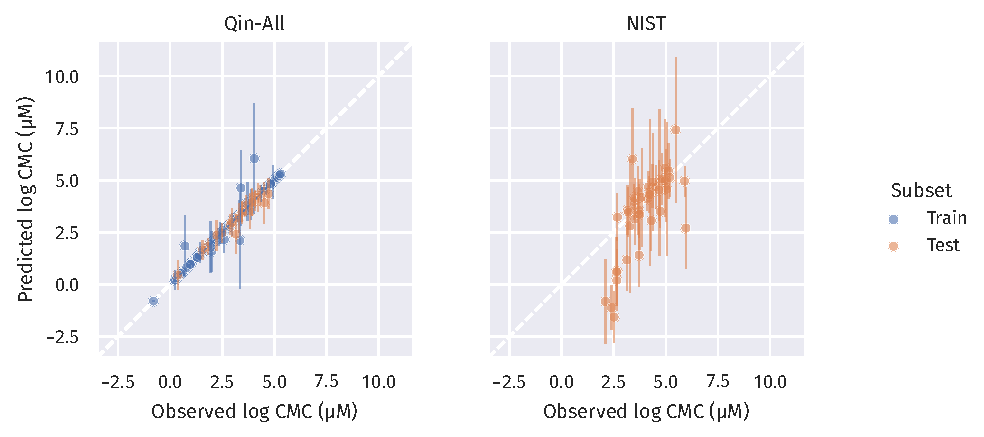
\includegraphics[width=\textwidth]{images/uq-parity.pdf}
        \caption{}
        \label{fig:uq-parity}
    \end{subfigure}
    \begin{subfigure}{\textwidth}
        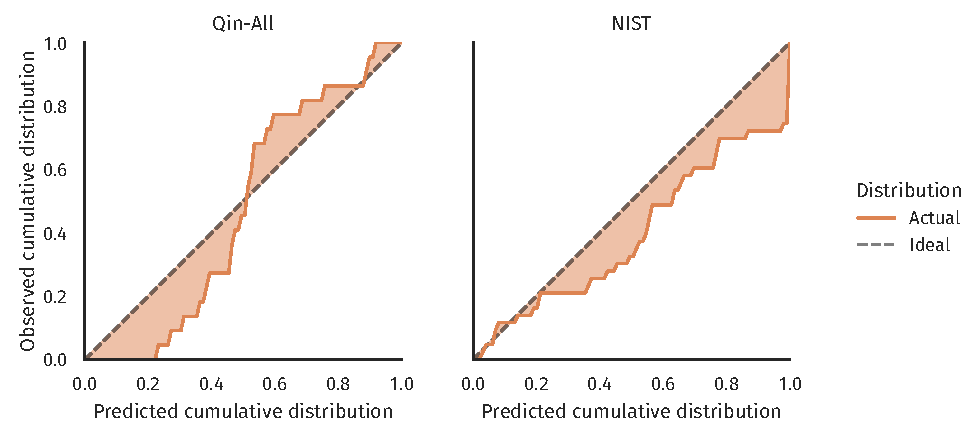
\includegraphics[width=\textwidth]{images/uq-calibration.pdf}
        \caption{}
        \label{fig:uq-calibration}
    \end{subfigure}
    \caption{(a) Parity plots of the predicted CMCs from the GNN/GP model and \SI{95}{\%}
        confidence intervals for the Qin-All and NIST datasets and (b)
        corresponding calibration plots for the test data predictions. The
        `ideal' distribution line indicates the cumulative distribution that
        would be obtained if residuals were drawn from the model's predicted
        distributions.}
\end{figure}

The S-shaped calibration curve for the Qin-All test data indicates that the
model was underconfident in its predictions. In fact, there is a spike in the
number of observed residuals that are close to the centre of the distribution.
The corresponding parity plot shows that the predicted uncertainties were
relatively small. The NIST data calibration curve's asymmetry indicates its
tendency to underestimate the CMCs. It shows a generally good agreement with the
ideal distribution, with the greatest discrepancy above \num{0.8}, which
indicates that there are several surfactants whose CMC predictions are too low
and that these predictions are overconfident, i.e. their predicted standard
deviations are too small.

\subsection{ECFP interpretations}

The weights of the ECFP models are coefficients corresponding to the scaled counts of the selected atomic environments. Referring to Equations \ref{eq:linear-ecfp} and \ref{eq:standard-scaling}, these coefficients indicate
the change in a predicted CMC when the count of $\mathcal{E}_m$ increases by $s_m$ from its average, $u_m$. A more readily interpreted value can be achieved by rescaling the coefficient, $w_m$, for an environment:
\begin{equation}
    w_m^\prime = \frac{w_m(1 - u_m)}{s_m},
\end{equation}
which indicates the difference in predicted CMC between a molecule containing
one $\mathcal{E}_m$ and a molecule without any $\mathcal{E}_m$, but which
otherwise contains exactly the same number as all the other environments. This
scaled weight can be interpreted as a rough indication of the relative
importance of different environments to determining CMC; `rough' because it may
not be physically plausible that two molecules exist that are distinguished only
by the number of $\mathcal{E}_m$ that they contain. This is particularly true of
larger environments that envelope smaller ones. The largest scaled weights for
the two ECFP models are given in Table \ref{tab:env-coefs}.

\begin{table}
    \centering
    \caption{The atomic environments with the greatest importance to CMC according to the trained ECFP models.}
    \label{tab:env-coefs}
    \begin{tabular}{@{}lSlS@{}} \toprule
        \multicolumn{2}{c}{Qin-All}                 & \multicolumn{2}{c}{Qin-Nonionics}                                                                                                                      \\\cmidrule(r){1-2}\cmidrule(l){3-4}
        Environment                                 & {Scaled weight}                   & Environment                                                                                      & {Scaled Weight} \\\midrule
        \ce{(CH2)5}                                 & -0.64                             & \ce{(CH2)5}                                                                                      & -0.76           \\
        \ce{(CH2)3}                                 & -0.55                             & \ce{(CH2)3}                                                                                      & -0.69           \\
        \ce{Cl-}                                    & 0.31                              & \chemfig{-[1]-[-1](-[-3]R_1)-[1]R_2}                                                             & -0.29           \\
        \ce{Br-}                                    & 0.29                              & \chemfig{R_1-[1](-[-1]R_3)-[3]R_2}                                                               & -0.25           \\
        \chemfig{R_1-[1]-[-1]-[1](-[3]R_2)-[-1]R_3} & -0.27                             & \chemfig{R_1-[1](-[4]R_2)(-[-2]R_3)-[1](-[3]OH)-[-1](-[-3]OH)-[1](-[3]OH)-[-1](-[-3]R_4)-[1]R_5} & -0.19           \\
        \ce{CH2}                                    & -0.23                             & \chemfig{R_1-[-1]-[1](-[3]OH)-[-1](-[-3]OH)-[1](-[3]OH)-[-1](-[-3]R_2)-[1]R_3}                   & 0.14            \\
        \ce{R1-O-R2}                                & 0.18                              & \chemfig{R_1-[-1](-[-3]R_2)-[1](-[3]OH)-[-1](-[-3]OH)-[1]-[-1]OH}                                & -0.12           \\
        \ce{OH}                                     & -0.17                             & \chemfig{R_1-[-1]-[1](=[3]O)-[-1](-[-3]OH)-[1](-[3]OH)-[-1]}                                     & 0.09            \\
        \ce{R1-O-(CH2)2OH}                          & -0.14                             & \ce{CH3}                                                                                         & -0.06           \\
        \ce{CH2-O-(CH2)2OH}                         & -0.14                             & \chemfig{R_1-[-1](-[-3]R_2)-[1](-[3]OH)-[-1](-[-3]OH)-[1](-[3]OH)-[-1](-[-3]R_3)-[1]R_4}         & 0.05            \\
        \bottomrule
    \end{tabular}
\end{table}

Both the Qin-Nonionic and Qin-All models agree that alkyl chain environments
constitute the top two most important contributors to CMC, suggesting that tail
length is the most important factor. The model trained on all surfactant classes
includes two counterions in its most important environments: \ce{Cl-} and
\ce{Br-}. This is to be expected; ionic surfactants typically have much larger
CMCs than nonionics, and the model appears to distinguish these by their
counterion. The Qin-Nonionics model identifies environments from the headgroups
of sugar-based surfactants as being important. These surfactant headgroups
possessed relatively complex topologies and therefore several environments; it
may have been necessary for the model to use many of these environments in order
to accurately distinguish between their CMCs.

\subsection{Applicability domain analysis}

Several of the molecules included in the NIST dataset were expected to be outside
of the applicability domain, which justifies their poor prediction accuracy. The
majority of the outliers' CMCs are underpredicted, and the GNN/GP model is
overconfident in their predictions. The 13 surfactants whose predictions'
residuals are greater than the \SI{95}{\%} confidence interval (CI) are shown in
Figure~\ref{fig:nist-underpred}. These constitute 3 nonionic surfactants, 1
zwitterionic surfactant and 9 ionic surfactants. Of the ionic surfactants, 5
have quaternary ammonium salts (quats) as counterions.

\begin{figure}
    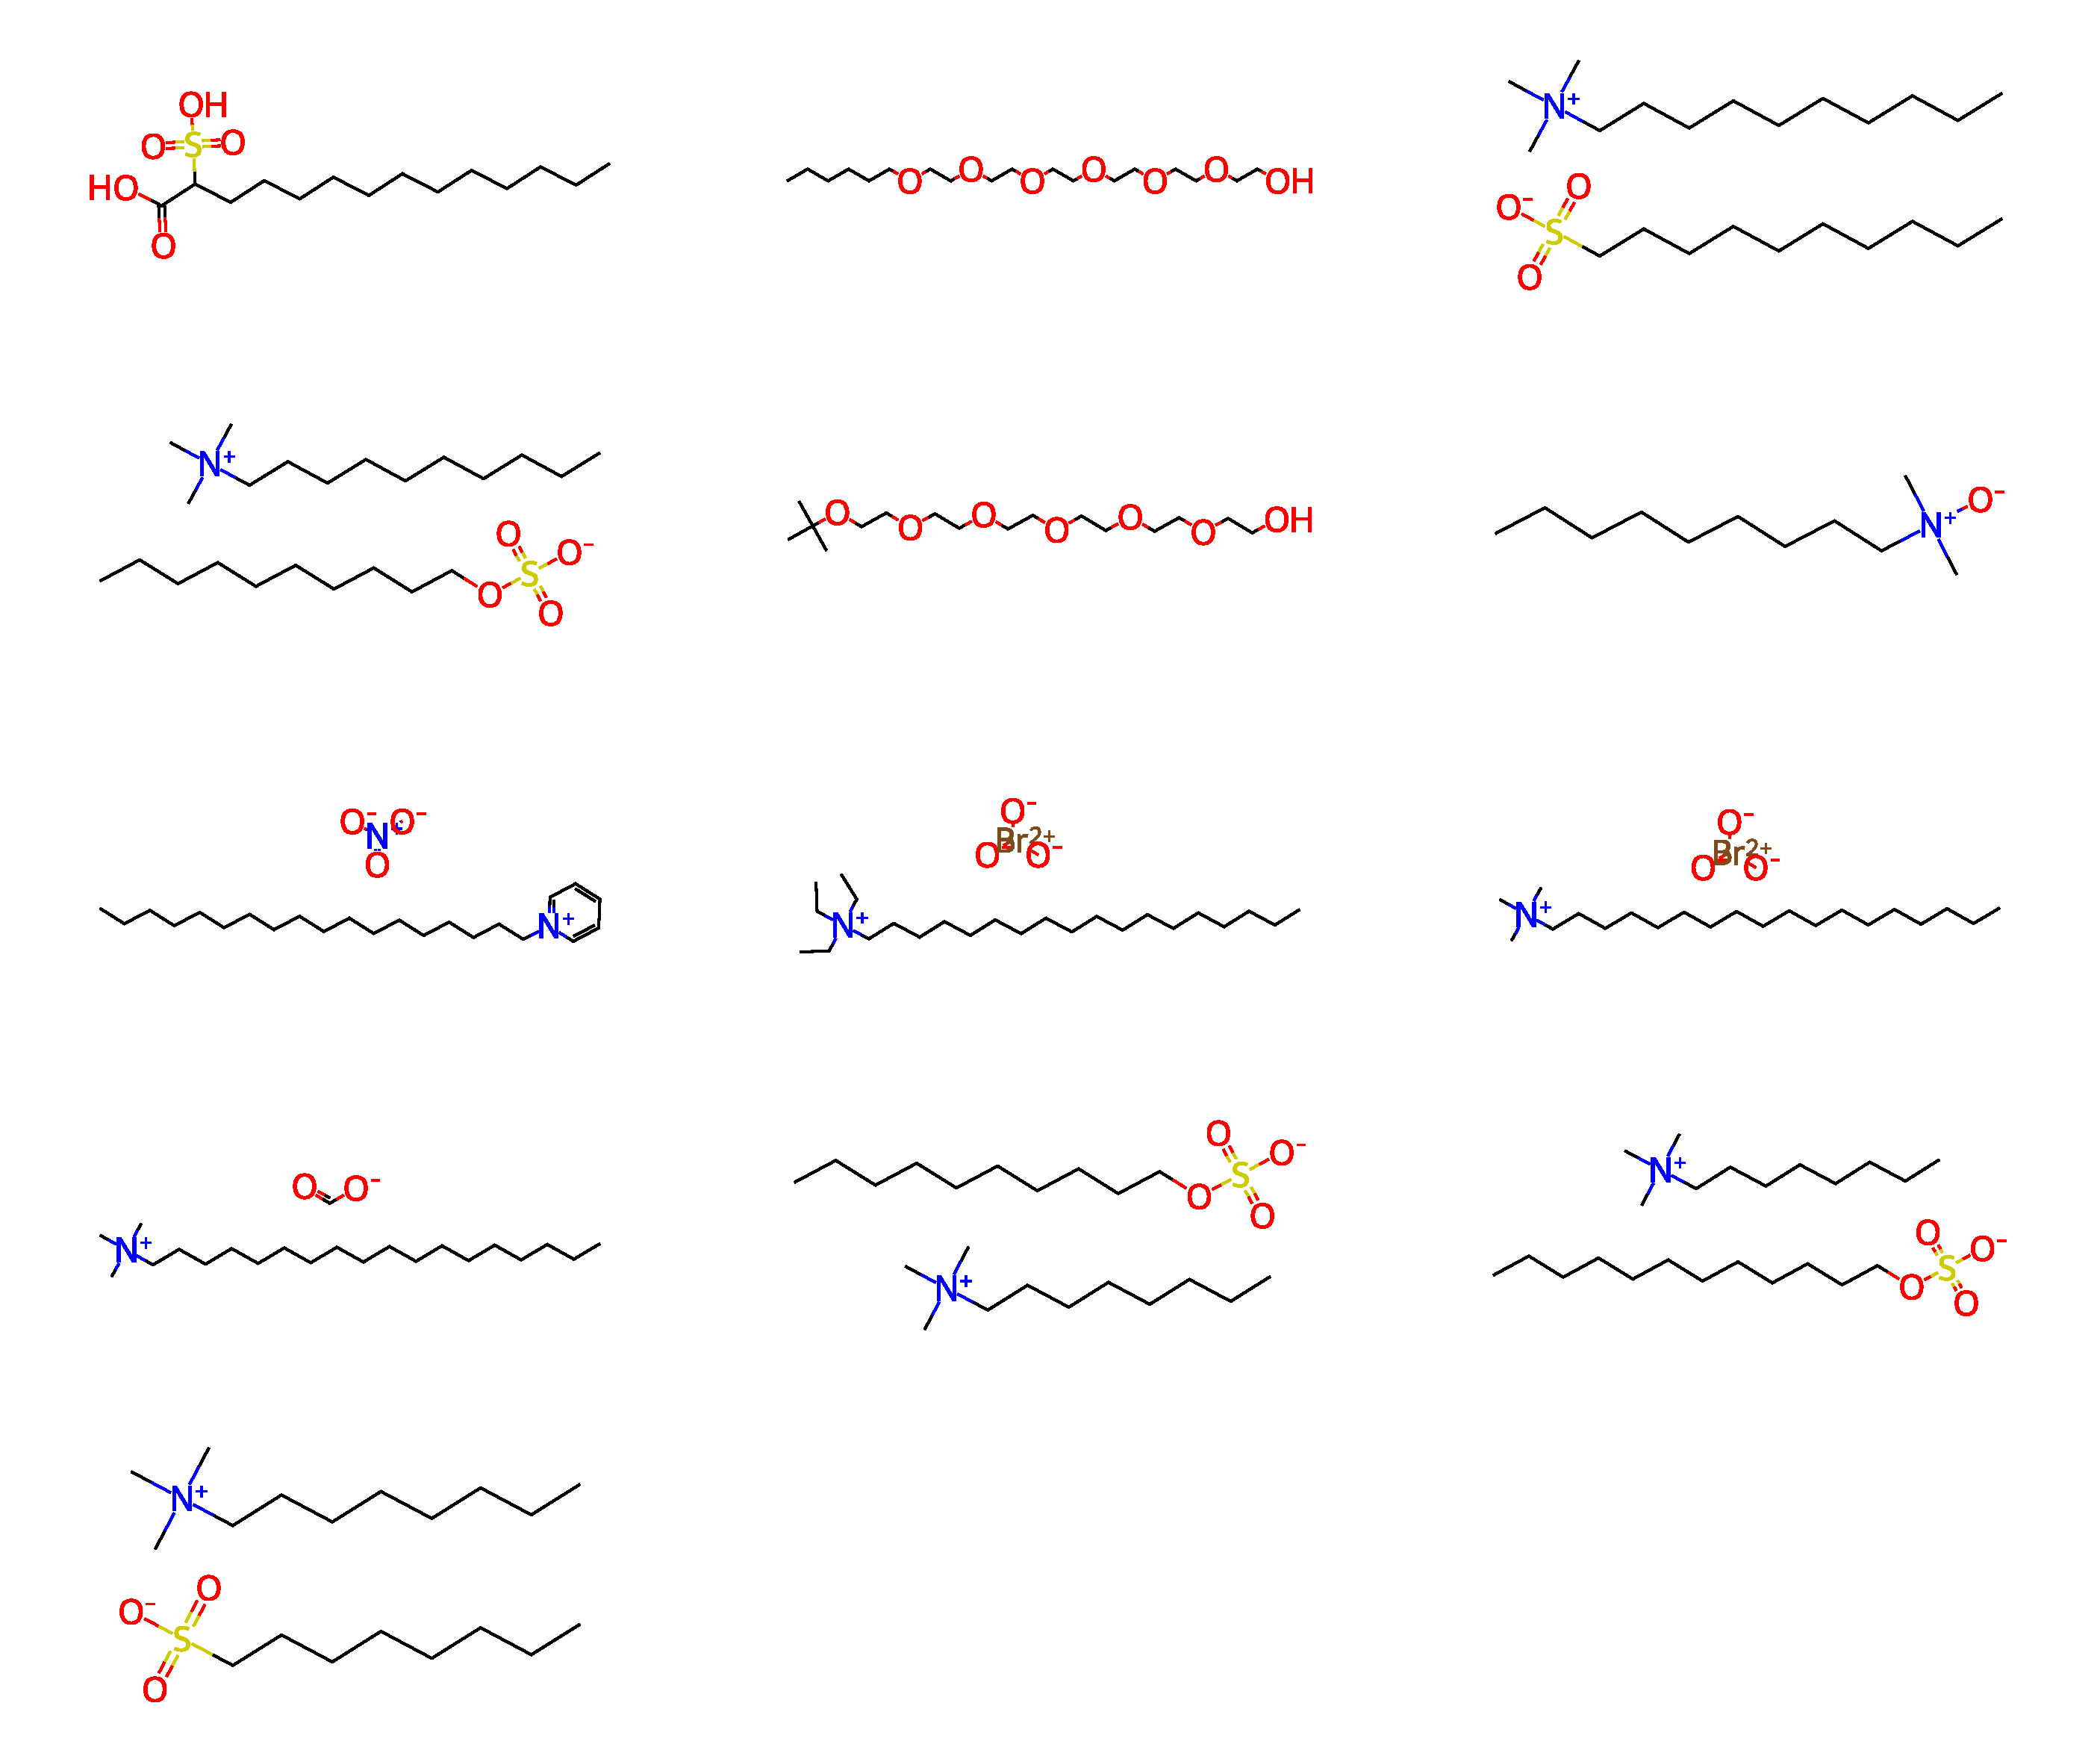
\includegraphics[width=\textwidth]{images/nist-underpred.pdf}
    \caption{The 13 surfactants and counterions in the NIST dataset with residuals
        that were greater than the \SI{95}{\%} confidence interval.}
    \label{fig:nist-underpred}
\end{figure}

It is useful to examine the types of counterions in these molecules as compared
to the training data. In the training data, there are no examples with a
bromate, nitrate or carboxylate counterion, but there are two examples of a quat
counterion. However, the quats in the training data are isotropic:
tetrapropylammonium and tetramethylammonium. In contrast, those that are
underpredicted are highly anisotropic and are effectively surfactants
themselves; the behaviour of these compounds, in terms of CMC, can be expected
to be very different to that of the surfactants in the training data.
Furthermore, the two polyoxyethylene alcohols in Figure~\ref{fig:nist-underpred}
have remarkably small tail groups relative to the examples in the training data,
which justifies their erroneous CMC predictions. This leaves two surfactants
among the outliers that might reasonably be expected to lie within the
applicability domain, constituting \SI{4.7}{\%} of the total NIST dataset, which
is close to the \SI{5}{\%} that are expected to be outside the \SI{95}{\%} CI.

To gain insight into the relationships between molecules, we exploit the kernel
function from the trained GP to create a molecular cartogram, as explained in
the Method. The resulting cartogram is shown in Figure~\ref{fig:fdg}. The NIST
molecules whose residuals are above the \SI{95}{\%} CI are also highlighted
separately.

From the cartogram of the entire data, it is apparent that the majority of the
surfactants are segregated based upon the type of counterion in the solution.
This suggests that the model has learned that the counterion is an important
factor for determining CMC and the weights associated with this counterion have
a profound impact on the CMC prediction. However, the visualisation of the NIST
molecules with CMCs above the \SI{95}{\%} CI indicates that the model classifies
all of these molecules as being primarily similar to the nonionic or
zwitterionic compounds. This is clearly erroneous for the ionic compounds: the
quats, the bromates, the carboxylates and the nitrates. This suggests that the
model has not learned appropriate weights for these counterions, hence it fails
to properly segregate them.

\begin{figure}
    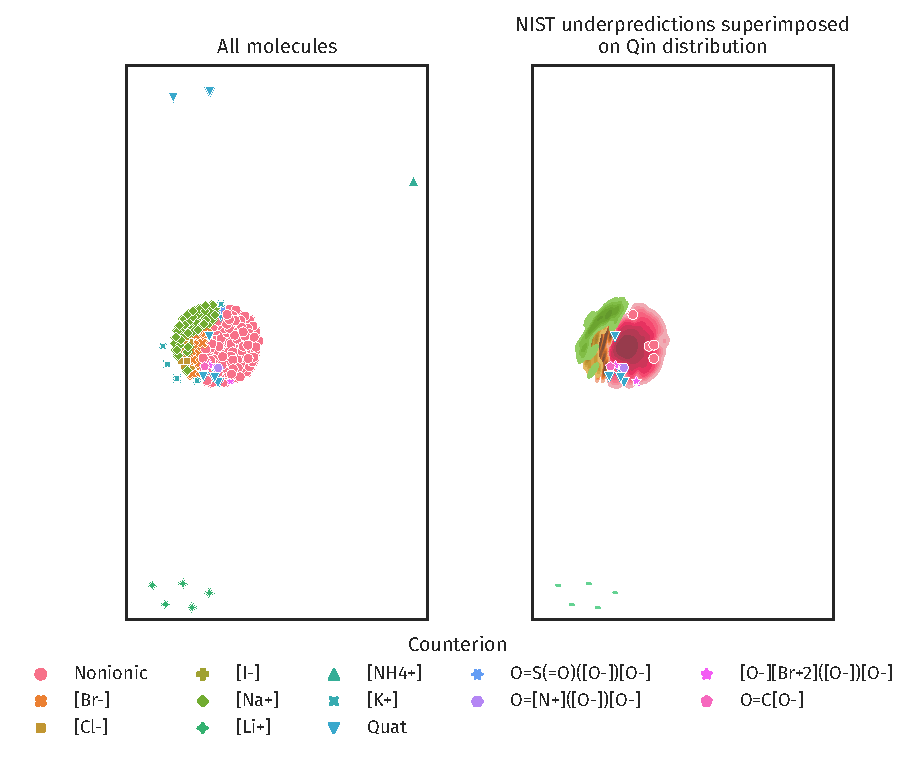
\includegraphics[width=\textwidth]{images/force-graph.pdf}
    \caption{Cartogram of the molecules in the combined NIST and Qin datasets
        using a force-directed graph layout. Left: The entirety of the combined
        NIST and Qin datasets, where each molecule is assigned a point. Right:
        The NIST molecules that are overconfidently underpredicted, so that the
        residual is above the \SI{95}{\%} confidence interval, are superimposed
        on a kernel density estimate (KDE) plot of the Qin data. This KDE plot
        is an estimate of the distribution of the Qin molecules on the left,
        coloured by the type of counterion.}
    \label{fig:fdg}
\end{figure}

\subsection{Sensitivity analysis}

Figure~\ref{fig:sensitivity} shows the test set evaluations for the GNN and ECFP
models using repeated, stratified $k$-fold cross-validation. The ECFP and GNN
models show very similar performance on the Qin-All dataset, but the ECFP model
outperforms the GNN model for all training ratios on the Qin-Nonionics dataset.
This is indicative of the propensity of neural networks to overfit, especially
on such small dataset sizes. Notably, there is also a much broader distribution
of RMSEs on the Qin-Nonionics data. This suggests that both of the Qin-Nonionics
models are much more sensitive to the specific molecules that are included in
the train and test splits.

Extrapolating the trend lines indicates that the benchmark performance is much
better than what would be expected. This highlights the importance of selecting
an appropriate training data split, which spans the entirety of the chemical
space of interest. On a dataset as small as the one used here, it is not
possible to achieve this without using a high training ratio.

\begin{figure}
    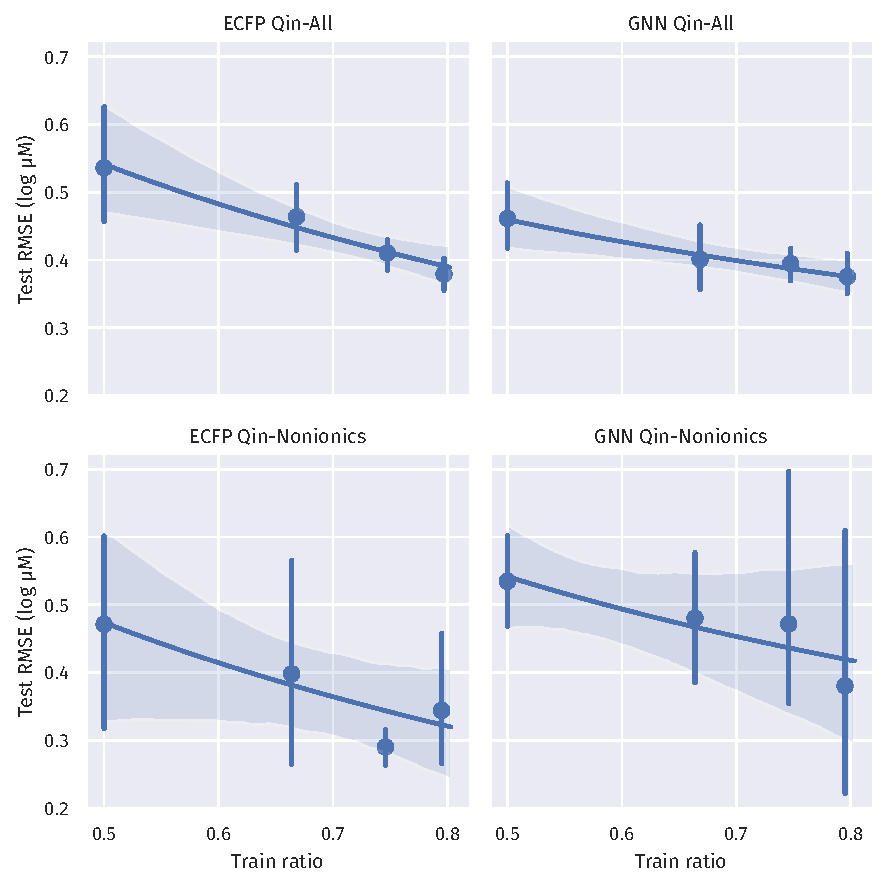
\includegraphics[width=\textwidth]{images/sensitivity-plots.pdf}
    \caption{Test set RMSEs for the sensitivity analysis models. The average
        RMSE for each value of $k$ is indicated, as well as the range of the RMSEs.
        A logarithmic fit to the data is shown, with a \SI{95}{\%} confidence
        interval determined by bootstrapping, using \num{1000} repeats.}
    \label{fig:sensitivity}
\end{figure}